\documentclass{vldb}
\usepackage{algorithm}
\usepackage{algorithmic}
\usepackage{amsfonts}
\usepackage{float}
\usepackage{tikz}
\usepackage{subfloat}
\usepackage[caption = false]{subfig}
\usepackage{amsmath}
\usetikzlibrary{datavisualization}
\usetikzlibrary{datavisualization.formats.functions}

\begin{document}

\title{(k,m)-Segmentation Algorithm for \\Horizontal Lines}
% ****************** AUTHORS **************************************

% You need the command \numberofauthors to handle the 'placement
% and alignment' of the authors beneath the title.
%
% For aesthetic reasons, we recommend 'three authors at a time'
% i.e. three 'name/affiliation blocks' be placed beneath the title.
%
% NOTE: You are NOT restricted in how many 'rows' of
% "name/affiliations" may appear. We just ask that you restrict
% the number of 'columns' to three.
%
% Because of the available 'opening page real-estate'
% we ask you to refrain from putting more than six authors
% (two rows with three columns) beneath the article title.
% More than six makes the first-page appear very cluttered indeed.
%
% Use the \alignauthor commands to handle the names
% and affiliations for an 'aesthetic maximum' of six authors.
% Add names, affiliations, addresses for
% the seventh etc. author(s) as the argument for the
% \additionalauthors command.
% These 'additional authors' will be output/set for you
% without further effort on your part as the last section in
% the body of your article BEFORE References or any Appendices.

\numberofauthors{2} %  in this sample file, there are a *total*
% of EIGHT authors. SIX appear on the 'first-page' (for formatting
% reasons) and the remaining two appear in the \additionalauthors section.

\author{

\alignauthor Lawrence P. Leipuner\\
       \affaddr{Brookhaven Laboratories}\\
       \affaddr{Brookhaven National Lab}\\
       \affaddr{P.O. Box 5000}\\
       \email{lleipuner@researchlabs.org}
% 5th. author
\alignauthor Sean Fogarty\\
       \affaddr{NASA Ames Research Center}\\
       \affaddr{Moffett Field}\\
       \affaddr{California 94035}\\
       \email{fogartys@amesres.org}
% 6th. author
}
\maketitle
\begin{abstract}
   
 Division of an electrical signals into high and low, cuts a soccer video into filed of game and audiences shots... all of those are a thresholding problems. But when the noise get stronger the regular thresholding algorithm get weaker . In the km-segment mean problem we need to divide an input signal into a k-piecewise function when each piece is one of set M in size m.

we aproximate the solution for a constrained version of $(k,m)$-segmentation problem when the lines are horizontal . We can do that by trying every m size set in the input data as M and compute the k-segment of the signal while limit the segment to be from M set. then choose the one with minimum cost. What give us $cost<4cost_opt$ by O(n chose m*…) time using corset tocompute k-segment (fl14 ).

we show how our algorithm can divides better than a regular threshold and keep divide when we increase the noises even after threshold totally failed.
\end{abstract}

\section{Introduction}
\subsection{Main Contribution}
The main contributions of the paper are: $(i)$ A solution for a constrained version of $(k,2)$-segmantation problem(as given in \ref{Problem Statement}) 
when the lines are horizontal .$(ii)$And to test this new solution on a Infra Red drone's conroler in order to do the first step of decoding this data.

\subsection{Problem Statement} \label{Problem Statement}
The $(k,m)$-segment mean problem optimally fits a given discrete time signal of $n$ points
by a set of $k$ linear segments over time,
where $k\geq1$ is a given integer. That is, we wish to
partition the signal into $k$ consecutive time intervals such that the points in each time
interval are lying on a single line from one of an $m$ types of lines, where $m\geq1$ is a given integer to;

We make the following assumptions with respect to the data:$(i)$ We assume the
data is represented by a feature space that suitably represents its underlying structure;
$(ii)$ The content of the data includes at most $k$ segments ,from at most $m$ (for this paper $m=2$) types. that we wish to detect auto-
matically; An example for this are scenes of the audience and the field in a soccer video, a "bits" of an Infra Red signal (as we show in Section \ref{Experimental Results}), etc. \\
This motivates the following problem definition.

\newdef{definition}{Definition}
\begin{definition}[$(k,m)$-segment mean]
A $set\ P\ in\ \mathbb{R}^{d+1} is\ a$ signal\\ 
$if\ P = \lbrace(1, p_1),(2, p_2),...,(n, p_n)\rbrace\ where\ p_i\in\mathbb{R}^d$ 
$is\ a\ point\ at\ time\ index\ i\ for\ evrey\\
i=[n]=\lbrace1,...,n\rbrace.$
$For\ an\ integers\ k\geq m\geq1,$
$a\ (k,m)-segmant\ is\ a\ k$-$picewise\ linear\ function:$
\[
f:\mathbb{R}\rightarrow\mathbb{R}^d = 
\begin{cases}
  \phantom{}f_1'(x) & \text{if}\ x<d_1 \\
  f_2'(x-d_1)        & \text{if}\ d_1x<d_2\\
  ...\\
  f_k'(x-d_{k-1})    & \text{if}\ d_{k-1}<x<d_k
\end{cases}
\]


where $\forall f_i : f_i' \in F,$ and $F$ is a group of lines from order $m$.
this fanction $f$ maps every time $i\in \mathbb{R}$ to a point $f(i)$ in $\mathbb{R}^d$.
\begin{figure}[H]

    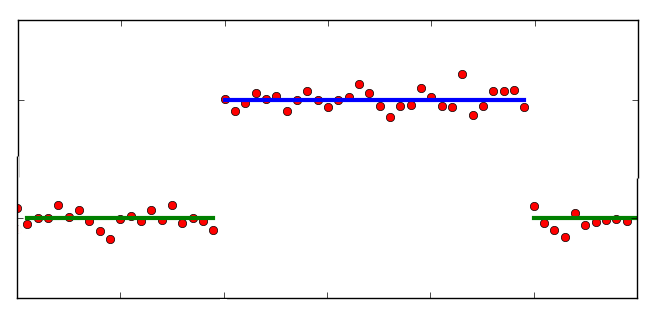
\includegraphics[width=0.5\textwidth]{12.png}
      \caption{This figure is an exemple to the $(3,2)$-segment. the red dots are the input data and the lines are the segments when the blue is the low type and the grin is the high type. 
      }
  \centering
\end{figure}

The fitting error at time $t$ is the squared distance
between $p_i$ and its corresponding projected point $f(i)$ on the $(k,m)$-segments.
The fitting cost of $f$ to $P$ is the sum of these squared distances.

\[
cost(P,f) = \sum_{i=1}^{n}\parallel p_i-f(i)\parallel_{2}^{2}.
\]

where $\parallel\cdot\parallel$ denotes the $Euclidean$ distance. 
The function $f$ is a $(k,M)$-segment mean of $P$ if it minimizes $cost(P,f)$ and conducts the conditions above.
\end{definition}

In this paper we interest in a constrained version of $(k,2)$-segmantation
($(k,m)$-segmantation for $m=2$) problem when the lines are horizontal.

\section{The algorithm}
If we lock at the problem we can see that $(i)$ if we had the corct set $F$
so the problem was esy sins all what we had to is to compute the $k$-segment(see Definition \ref{k-segment}) mean wehn eatch segmant is in $F$.$(ii)$ And if we had the dividers of the segments on the $(k,m)$-segmat then each segment
will be the mean height of the corresponding input points. 

\begin{definition}[$k$-segment mean] \label{k-segment}
The $k$-segment mean problem is a private case of the $(k,m)$-segment mean, when $k = m$.

\end{definition}


\begin{definition}[Bicriteria or $(\alpha,\beta)$-approximation]
For $ \alpha, \beta > 0$, an $(\alpha, \beta)-approximation$ for the $(k,m)-segment mean$
 of $P$ is a $(k · β)-segment$ $ g$ such that $cost(P, g) \leq \alpha \ast cost(P, f ∗).$

\end{definition}

\newtheorem{theorem}{Theorem}
\begin{theorem}[Bicriteria approximation~\cite{FL11}]
Let $P=\lbrace(1, p_1),...,(k, p_k)\rbrace$. Then an $(\alpha,\beta)$-approximation for $P$ can be computed in $O(dn)$ time where $\alpha=..$ and $\beta=..$

\end{theorem}

For this solution to the km-segment problem we use 
$i)$ Bicriteria.
$ii)$ BalancedPartition.
As described in Feldman's 2014.


\begin{algorithm}
\begin{algorithmic}
\STATE \textbf{Input:} A set $P = \lbrace(1,p_1),...,(n,p_n)\rbrace$ in $ \mathbb{R}^{d+1}$
and integer $k\geq1$
\STATE \textbf{Output:} A $2$-approximation to the $(k,m)$-segment mean of $P$\\ when $m=2$.
 
Set $a\gets \infty$
\FOR {$\lbrace p_i,p_j\in P\vert 1\leq i\leq j\leq n  \rbrace$} 

\STATE 
Set $f \gets Bicriteria(P,k,p_i,p_j)$ \\
$coreset = BalancedPartition(P,\varepsilon,cost(f),p_i,p_j)$\\
$temp=K$-$Segmentation(coreset,k,p_i,p_j)$\\
\STATE $best\_fit = $ Compute $temp$ such that $cost(P,temp)$ is minimized.

\ENDFOR

\RETURN $best\_fit$



\caption{km - segmentation main}

\end{algorithmic}
\end{algorithm}
$g_i$ is the line $y= p_i$
\begin{algorithm}
\begin{algorithmic}
\STATE Input: A set $P\subseteq \mathbb{R}^{d+1}$
and two vectors $p_1,p_2 \in \mathbb{R}^d$
\STATE Output: An $2$-approximation to the $(k,m)$-segment mean of P when $m=2$.
\IF {$cost(g_1,P) < cost(g_2,P))$}
\RETURN $g_1$
\ELSE
\RETURN $g_2$
\ENDIF 

\caption{alternative for 1 - segment main}

\end{algorithmic}
\end{algorithm}\\
\newtheorem{A}{Theorem}
\begin{theorem}[solution cost]
This algorithm that we present will give a $f'$ that 
$cost(P,f')\leq (2+\varepsilon)*cost(P,f)$
\\


\end{theorem}
\begin{proof}
Without loss of generality
if we lock on all of the dots on the segments that from the higher type .
Let $p_{opt}$ be the men of the corresponding of all those points, Let $cost_{opt}$ be the averege distance to $p_{opt}$ and let $p_{s}$ be the closest point to $p_{opt}$.Then the distanse $\Delta(p_{opt},p_s)$ is smoler or equal to $cost_{opt}$ so from the triangle inequality for each point $p$ in the data: $\Delta(p,p_s)<2*cost_{opt}$ ($\Delta(p,p_{opt})+\Delta(p_{opt},p_s)$).

\end{proof}

\section{Experimental Results} \label{Experimental Results}
We now demonstrate the results of our algorithm on sintetic data in cuple of tests. We compare our algorithms against regular thresholding algorithem. we also show our algorithim preformens on a real life data token from an ir remote controlers.

\begin{figure}[H]
\centering
\subfloat[Normal noise varians vs erorr]{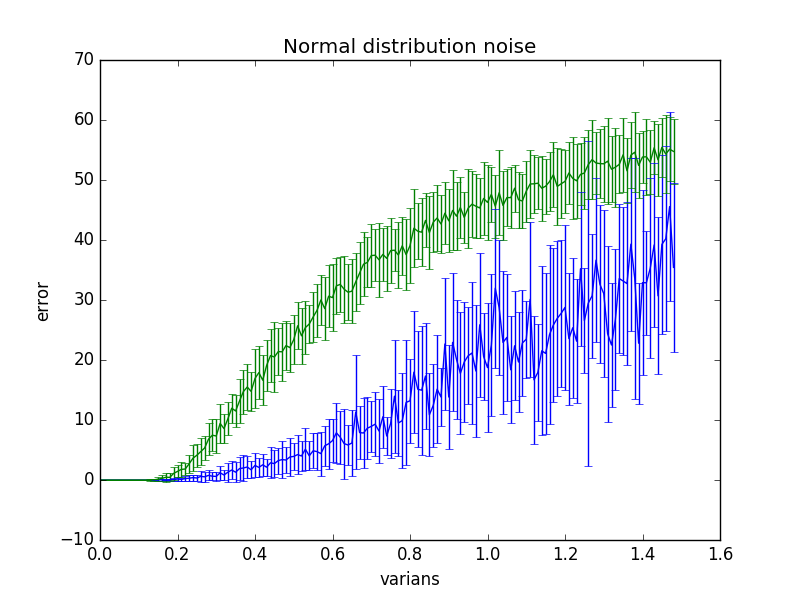
\includegraphics[width=0.5\textwidth]{normal_f.png}} \\
\subfloat[Uniform noise varians vs erorr]{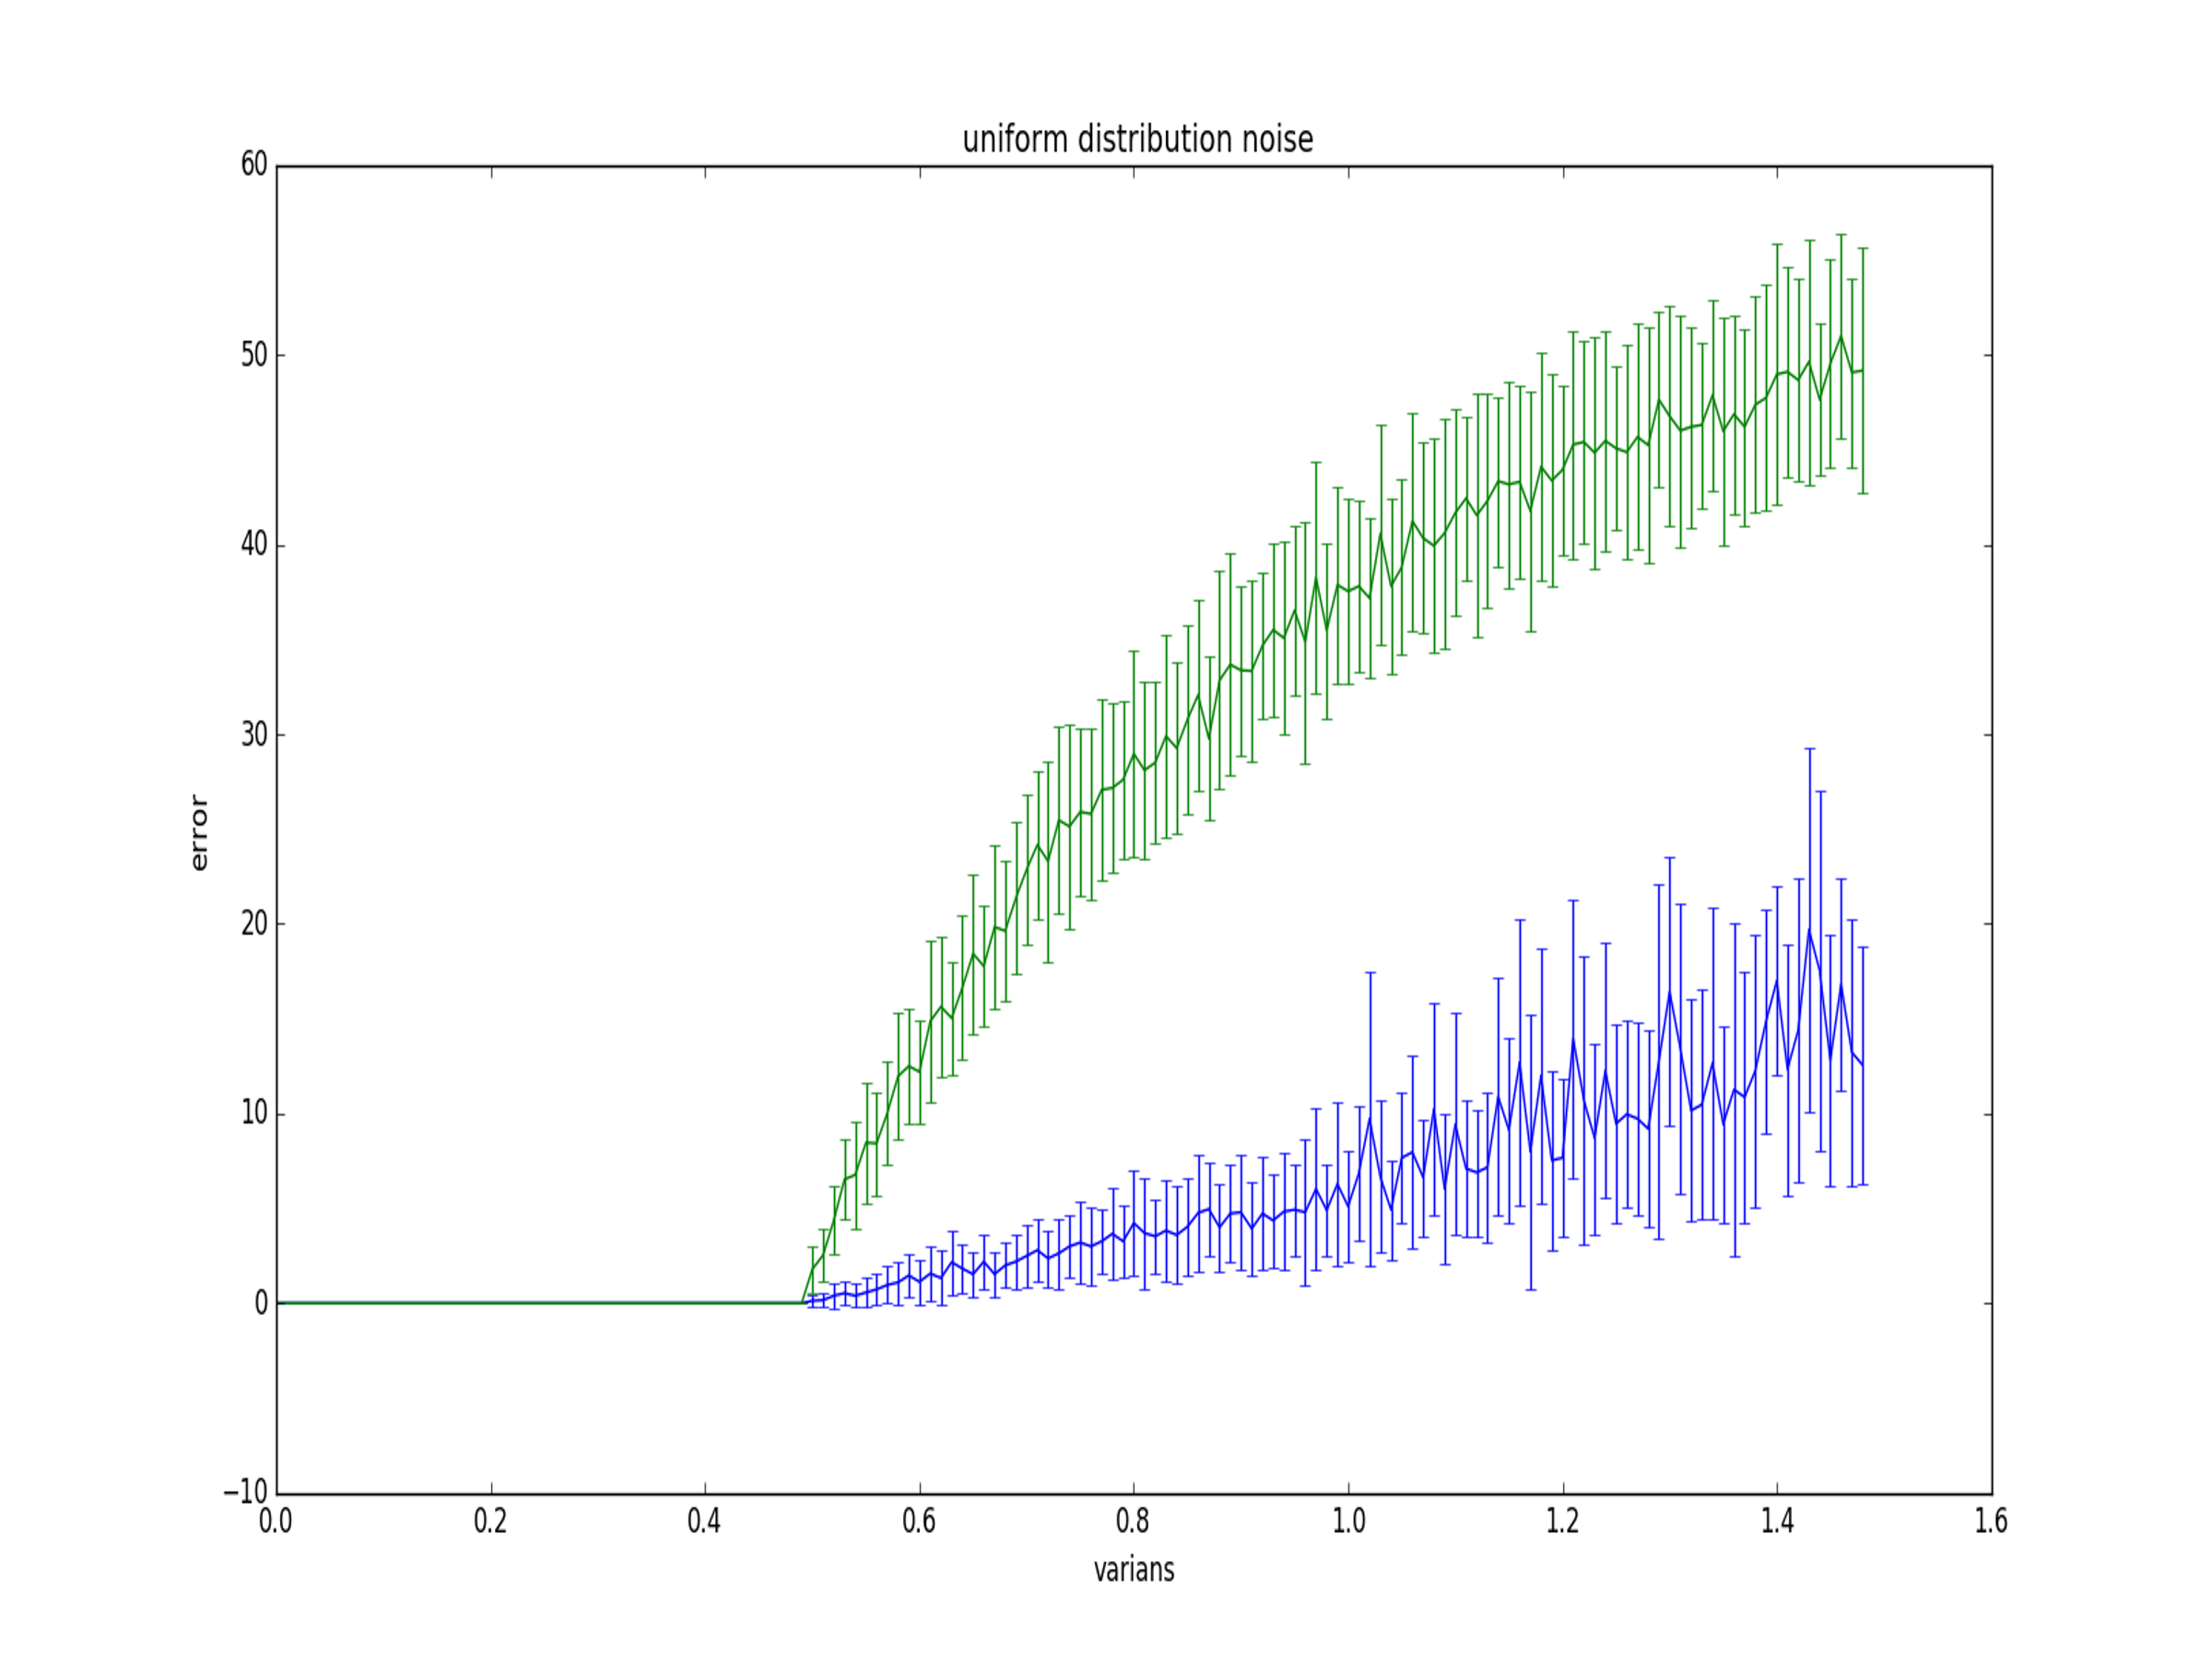
\includegraphics[width=0.5\textwidth]{uni_f.png}}\\
\centering\subfloat[Number of segment vs erorr]{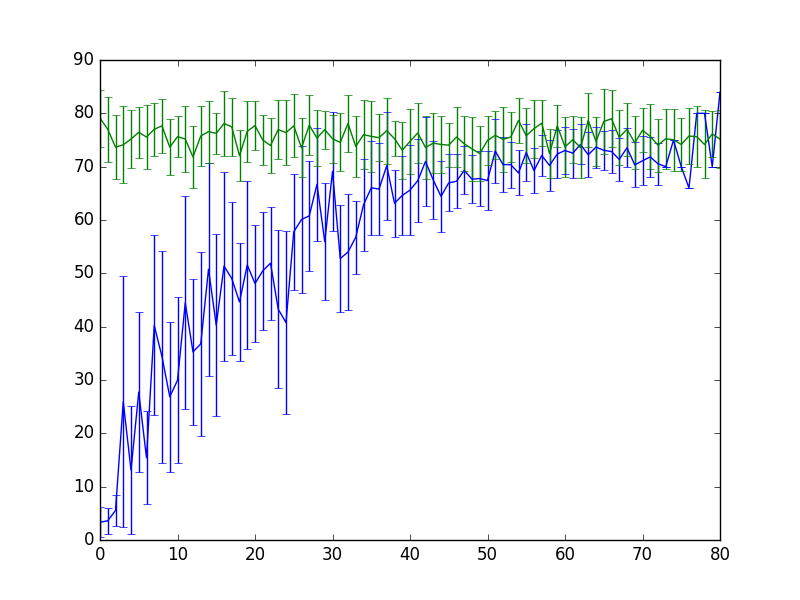
\includegraphics[width=0.5\textwidth]{figure_1-3.png}}
\caption{Figure 2a shows the division error as fanction of normal noise varians that added to the signal. For $(k,m)$-segmantation algorithim(blue) against threshold's(green). Figure 2b shows the same as 2a but for a uniform noise. Figure 2c shows the division error as fanction of the number of segments in the input signal $(k,m)$-segment(blue) against  thresholding(green).  }
\label{noise}
\end{figure}
\subsection{segmantation of data}
We first examine the behavior of the algorithm on synthetic data which provides us with
easy ground-truth, to evaluate the quality of the algorithem.We generate synthetic test data by drawing a discrete $(k,m)$-segment $P$ whith $k=15$ and $m=2$, and then we add Gaussian and normal noise(one in eatch experament).


\begin{figure}[H]
\centering
\subfloat[IR controler to IR resiver distance vs erorr]{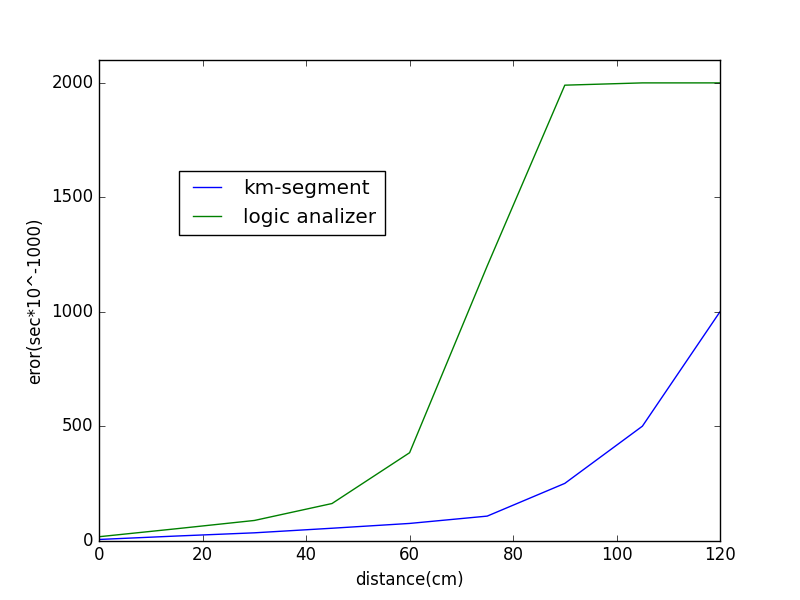
\includegraphics[width=0.5\textwidth]{Experimental.png}}  \\
\subfloat[IR controler to IR resiver distance vs erorr]{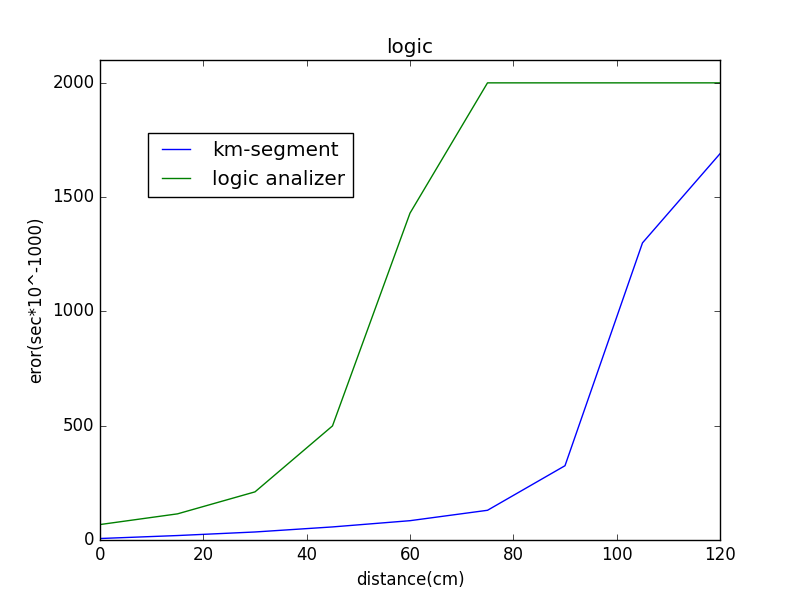
\includegraphics[width=0.5\textwidth]{ir2.png}}\\

\caption{Figures 3a and 3b shows the resultes of the expermaente that discribe in subsection \ref{IR} .the graphs shows taht the incrising of the division error($\mu sec$) of the $(k,m)$-egmantation(blue) is slower  the incrising of the logic analizer(green) division error while we increse the distance between the IR controler and the IR resever($cm$),for two diffrent key configurations .}
\end{figure}
\subsection{real life data}\label{IR}
We compare our algorithem agense Logic-analizer divice. We conect an IR reciver circal that plot anlog sinal to the Logic-analizer and then ww comper the Logic 
\medskip

\begin{thebibliography}{9}
\bibitem{FL11} 
D . Feldman, G. Rosman, M. Volkov, J.W. Fisher III, and D. Rus
Proc. 
\textit{Coresets for $k$-Segmentation of Streaming Data}. 
27th Conference on Neural Information Processing Systems (NIPS) 2014
 
\end{thebibliography}
\end{document}
